% NeurIPS 2026 format — Learning to Reweight Examples (Bonus Assignment)
% Template: https://www.overleaf.com/latex/templates/formatting-instructions-for-neurips-2026/bjdwqfdkyftc

\documentclass{article}

% --- NeurIPS 2026 packages (use neurips_2026.sty if available) ---
\usepackage[final]{neurips_2026}   % fallback to 2024 style
\usepackage[utf8]{inputenc}
\usepackage[T1]{fontenc}
\usepackage{hyperref}
\usepackage{url}
\usepackage{booktabs}
\usepackage{amsfonts}
\usepackage{amsmath}
\usepackage{amssymb}
\usepackage{nicefrac}
\usepackage{microtype}
\usepackage{graphicx}
\usepackage{subfigure}
\usepackage{xcolor}
\usepackage{algorithm}
\usepackage{algorithmic}
\usepackage{multirow}
\usepackage{fancyhdr}
\pagestyle{fancy}
\fancyhf{}
\renewcommand{\headrulewidth}{0pt}
% \renewcommand{\headrulewidth}{0pt}
% \makeatletter
% \def\ps@headings{%
%   \def\@oddhead{}%
%   \def\@evenhead{}%
%   \def\@oddfoot{\hfil\thepage\hfil}%
%   \let\@evenfoot\@oddfoot}
% \makeatother
\title{Replicating ``Learning to Reweight Examples for Robust Deep Learning''}

\author{
  Nishanth Senthil Kumar \\
  Roll No: EE23B049 \\\
  \texttt{ee23b049@smail.iitm.ac.in}
}

\begin{document}
\maketitle

% ─────────────────────────────────────────────────────────────
\begin{abstract}
This work replicates and extends the meta-learning example reweighting algorithm
proposed by Ren et al.\ (2018), ``Learning to Reweight Examples for Robust Deep
Learning'', on two standard UCI benchmark datasets.
The original paper frames training-set bias correction as a bi-level optimisation
problem, dynamically assigning importance weights to training examples by
matching their gradient directions to those of a small, clean validation set.
We implement the algorithm using a NumPy multi-layer perceptron with
second-order automatic differentiation and evaluate it against three course
baselines (Logistic Regression, Random Forest, SVM) under controlled class-imbalance
ratios (2:1 to 20:1) and label-noise rates (0\%–50\%, uniform and background flip).
Our experiments confirm the paper's core claim: L2RW assigns significantly lower
weights to corrupted examples, helping the model avoid noise over-fitting.
However, we observe that the MLP-based L2RW is outperformed by well-tuned
ensemble methods on structured tabular data, highlighting an important
practical limitation.
Code is available at \url{https://github.com/lazarsalt14/DA5400-Project/tree/main/l2rw}.
Video presentation: \url{https://youtu.be/xU3EYTdYbQw}.
\end{abstract}

% ─────────────────────────────────────────────────────────────
\section{Motivation}

Modern supervised machine learning pipelines routinely encounter two forms of
training-set bias: \emph{class imbalance} and \emph{label noise}.
Class imbalance arises when one class dominates the training distribution, a
common problem in fraud detection, medical diagnosis, and rare-event prediction.
Label noise is introduced whenever annotations are collected cheaply, for
example through crowd-sourcing or weakly supervised sources, and corrupted
labels can cause a neural network to memorise incorrect patterns and
generalise poorly \citep{zhang2017rethinking}.

Classical remedies, which include inverse-frequency weighting, balanced resampling, assume a fixed definition of ``good'' examples.
In noisy label settings, high-loss examples are typically corrupted and should
be \emph{down-weighted}, yet in class-imbalance settings the same high-loss
examples belong to the rare class and should be \emph{up-weighted}.
When both biases co-exist, these heuristics become fundamentally inconsistent.

Ren et al.\ (2018) propose a principled, assumption-free alternative: let the
model learn to assign weights to training examples online, guided by a small
held-out set of clean, unbiased validation data.
The motivating insight is elegant, a training example should receive a high
weight if and only if it improves performance on the clean validation set.
This assignment is achieved without any additional hyperparameters by
computing the gradient similarity between each training example and the
validation set at every training step.

The problem is highly relevant today: large-scale datasets used to train
foundation models are frequently assembled from noisy internet sources
\citep{russakovsky2015imagenet}, and practitioners need principled methods to
re-weight or filter such data without expensive manual verification.

% ─────────────────────────────────────────────────────────────
\section{Problem Statement}

\subsection{Notation}

Let $\mathcal{D}_f = \{(x_i, y_i)\}_{i=1}^N$ be a potentially biased training
set (imbalanced or noisy labels) and
$\mathcal{D}_g = \{(x_j^v, y_j^v)\}_{j=1}^M$ be a small, clean validation set
with $M \ll N$.
Let $\Phi(x; \theta)$ be a neural network with parameters $\theta$, and
$C(\hat{y}, y)$ the cross-entropy loss.

\subsection{Standard vs Reweighted Training}

Standard empirical risk minimisation minimises
$\frac{1}{N}\sum_{i=1}^{N} C(\Phi(x_i;\theta), y_i)$,
treating all examples equally.
The L2RW objective instead solves the \emph{bi-level} optimisation:

\begin{equation}
  w^* = \argmin_{w \geq 0} \; \frac{1}{M} \sum_{j=1}^{M}
        C\bigl(\Phi(x_j^v;\,\theta^*(w)),\, y_j^v\bigr),
  \label{eq:bilevel-outer}
\end{equation}

\begin{equation}
  \theta^*(w) = \argmin_\theta \; \sum_{i=1}^{N} w_i\,
                C\bigl(\Phi(x_i;\theta),\, y_i\bigr),
  \label{eq:bilevel-inner}
\end{equation}

where $w = \{w_i\}_{i=1}^N$ are the per-example weights.

\subsection{Online Approximation}

Solving Equations~\eqref{eq:bilevel-outer}--\eqref{eq:bilevel-inner} exactly
requires two nested optimisation loops, which is computationally prohibitive.
The key insight of the paper is to approximate the optimal weights at each
training step $t$ using a single gradient step.
Given a training mini-batch $\{(x_i, y_i)\}_{i=1}^n$ and validation
mini-batch $\{(x_j^v, y_j^v)\}_{j=1}^m$, the unnormalised weight for
example $i$ is:

\begin{equation}
  u_{i,t} = -\frac{\partial}{\partial \varepsilon_i}
             \frac{1}{m}\sum_{j=1}^m
             f_j^v\!\bigl(\hat\theta_{t+1}(\varepsilon)\bigr)\bigg|_{\varepsilon=0},
  \label{eq:meta-grad}
\end{equation}

where $\hat\theta_{t+1}(\varepsilon) = \theta_t -
\alpha \nabla \sum_i \varepsilon_i f_i(\theta_t)$
is a one-step lookahead with perturbed weights $\varepsilon$.

For a multi-layer perceptron with $L$ layers, activations
$\tilde{z}_{l}$ and gradients $g_l$, Equation~\eqref{eq:meta-grad}
simplifies to:

\begin{equation}
  u_{i,t} \;\propto\;
  -\frac{1}{m}\sum_{j=1}^{m}\sum_{l=1}^{L}
  \underbrace{(\tilde{z}_{j,l-1}^v{}^\top \tilde{z}_{i,l-1})}_{\text{activation similarity}}
  \underbrace{(g_{j,l}^v{}^\top g_{i,l})}_{\text{gradient similarity}}.
  \label{eq:similarity}
\end{equation}

Intuitively, a training example is helpful (and should be up-weighted) if its
per-layer activations and gradient directions align with those of the clean
validation set.

Weights are rectified and normalised:

\begin{equation}
  \tilde{w}_{i,t} = \max(u_{i,t}, 0), \qquad
  w_{i,t} = \frac{\tilde{w}_{i,t}}{\sum_j \tilde{w}_{j,t} + \delta(\sum_j \tilde{w}_{j,t})},
  \label{eq:normalise}
\end{equation}

where $\delta(a) = \mathbf{1}[a=0]$ prevents the degenerate all-zero case.

\subsection{Convergence}

(Quoting this directly from the paper), Under mild conditions (Lipschitz-smooth validation loss, $\sigma$-bounded
training gradients, learning rate $\alpha_t \leq \frac{2n}{L\sigma^2}$),
the validation loss decreases monotonically and the algorithm converges to
a critical point at rate $O(1/\sqrt{T})$, the same rate as SGD.

% ─────────────────────────────────────────────────────────────
\section{Datasets}

We use two synthetic datasets generated from \texttt{sklearn.datasets.make\_classification},
designed to mimic the statistical properties of real UCI imbalance and noise benchmarks.

\paragraph{Dataset 1, Credit (class imbalance).}
This dataset simulates a credit-card fraud detection scenario.
It contains $N=2{,}000$ samples with 20 features (10 informative, 4 redundant),
drawn from a binary classification problem.
We systematically vary the majority-to-minority class ratio
$r \in \{2, 5, 10, 15, 20\}$, mirroring the imbalance ratios studied in
Section~4.1 of the paper.
At ratio 20:1 the minority class constitutes only $\sim\!5\%$ of training data,
a realistic setting for fraud detection.
The dataset is split into 70\% training, 10\% clean validation, and 20\% test.
The validation and test sets are class-balanced (stratified split).

\paragraph{Dataset 2, Phishing (noisy labels).}
This dataset simulates a phishing-website classification problem.
It contains $N=2{,}000$ samples with 15 features and 4 balanced classes.
We inject two types of synthetic label noise at rates
$r \in \{0, 10, 20, 30, 40, 50\}\%$:
\begin{itemize}
  \item \textbf{Uniform flip}: each noisy label is replaced by a uniformly
    random different class, corresponding to Table~1 of the paper.
  \item \textbf{Background flip}: all noisy labels are mapped to class 0
    (background), corresponding to Table~2 of the paper and modelling the
    common scenario where positive instances are missed during annotation.
\end{itemize}
The validation set (10\%) uses clean labels; only the training labels are corrupted.

Both datasets are small enough to run on a standard CPU, making the experiments
fully reproducible without specialised hardware.

% ─────────────────────────────────────────────────────────────
\section{Experimental Setup and Baselines}

\subsection{L2RW Implementation}

We implement L2RW using a two-hidden-layer MLP (64--32 units, ReLU activations,
softmax output) in pure NumPy with He initialisation.
The gradient similarity in Equation~\eqref{eq:similarity} is computed
explicitly without automatic differentiation frameworks.
Hyperparameters: learning rate $\alpha=0.25$, 200 epochs,
batch size $n=64$, validation batch size $m=|D_g|$.
Standard scaler is applied to all inputs.

\subsection{Three Course Baselines}

\begin{enumerate}
  \item \textbf{Logistic Regression (LR)}: $\ell_2$-regularised LR from
    \texttt{sklearn}, with both uniform and balanced class weighting.
    Represents a well-understood linear decision boundary.

  \item \textbf{Random Forest (RF)}: 200-tree ensemble with Gini impurity.
    Chosen for its robustness to irrelevant features and its built-in
    feature importance mechanism.

  \item \textbf{Support Vector Machine (SVM)}: RBF kernel SVM with
    probability calibration via Platt scaling.
    Maximises the margin and is known to handle moderate class imbalance
    better than MLP-based methods.
\end{enumerate}

All sklearn baselines are tested with both default and \texttt{class\_weight="balanced"}
settings, and scaled with \texttt{StandardScaler}.

\subsection{Additional MLP Comparisons}

Following the paper, we also compare against:
\begin{itemize}
  \item \textbf{Vanilla MLP}: the same architecture as L2RW, trained without reweighting.
  \item \textbf{PROPORTION}: inverse-frequency weighting of training losses.
  \item \textbf{RESAMPLE}: class-balanced oversampling of the training set.
\end{itemize}

% ─────────────────────────────────────────────────────────────
\section{Evaluation Metrics}

We evaluate all methods on the held-out test set using:

\begin{itemize}
  \item \textbf{Accuracy}: overall classification accuracy.
    Can be misleading under class imbalance, but included for comparability.

  \item \textbf{F1 Macro}: unweighted mean of per-class F1 scores.
    Penalises poor performance on minority classes equally.
    Primary metric for imbalance experiments.

  \item \textbf{AUC-ROC (macro OvR)}: area under the receiver operating
    characteristic curve, averaged over classes via one-vs-rest.
    Measures ranking quality, less sensitive to threshold choice.

  \item \textbf{G-mean}: geometric mean of per-class recalls.
    Zero if any class has zero recall; ideal metric for severe imbalance.
\end{itemize}

For multi-class problems (noise experiment), binary AUC is extended to
the macro one-vs-rest (OvR) formulation.

% ─────────────────────────────────────────────────────────────
\section{Results}

\subsection{Experiment 1: Class Imbalance}

Table~\ref{tab:imbalance} reports the F1 Macro score of all methods across
five imbalance ratios on the Credit dataset.

\begin{table}[h]
\centering
\caption{F1 Macro on Credit dataset. Best per-column in \textbf{bold}.}
\label{tab:imbalance}
\resizebox{\columnwidth}{!}{%
\begin{tabular}{lcccccc}
\toprule
\textbf{Model} & \textbf{2:1} & \textbf{5:1} & \textbf{10:1} & \textbf{15:1} & \textbf{20:1} \\
\midrule
Logistic Reg           & 0.861 & 0.802 & 0.697 & 0.668 & 0.713 \\
LR (balanced)          & 0.861 & 0.808 & 0.707 & 0.660 & 0.615 \\
Random Forest          & 0.904 & 0.859 & 0.700 & 0.707 & 0.626 \\
RF (balanced)          & 0.898 & 0.856 & 0.710 & 0.681 & 0.584 \\
SVM                    & 0.937 & 0.910 & 0.788 & 0.754 & 0.664 \\
\textbf{SVM (balanced)}& \textbf{0.937} & \textbf{0.936} & \textbf{0.839} & \textbf{0.782} & \textbf{0.884} \\
Vanilla MLP            & 0.930 & 0.889 & 0.860 & 0.763 & 0.732 \\
MLP + PROPORTION       & 0.939 & 0.892 & 0.849 & 0.759 & 0.826 \\
MLP + RESAMPLE         & 0.925 & 0.915 & 0.839 & 0.756 & 0.795 \\
L2RW (ours)            & 0.902 & 0.827 & 0.827 & 0.695 & 0.642 \\
\bottomrule
\end{tabular}}
\end{table}

Figure~\ref{fig:imbalance} plots F1 against imbalance ratio.
SVM with balanced weighting shows the largest resilience, achieving
$\mathrm{F1}=0.884$ at the hardest 20:1 setting.
The L2RW MLP shows competitive performance at moderate ratios (10:1, F1=0.827)
but is not the top performer, likely due to the small validation set size
(only 9 minority-class examples at 20:1) limiting the meta-gradient signal.

\begin{figure}[h]
  \centering
  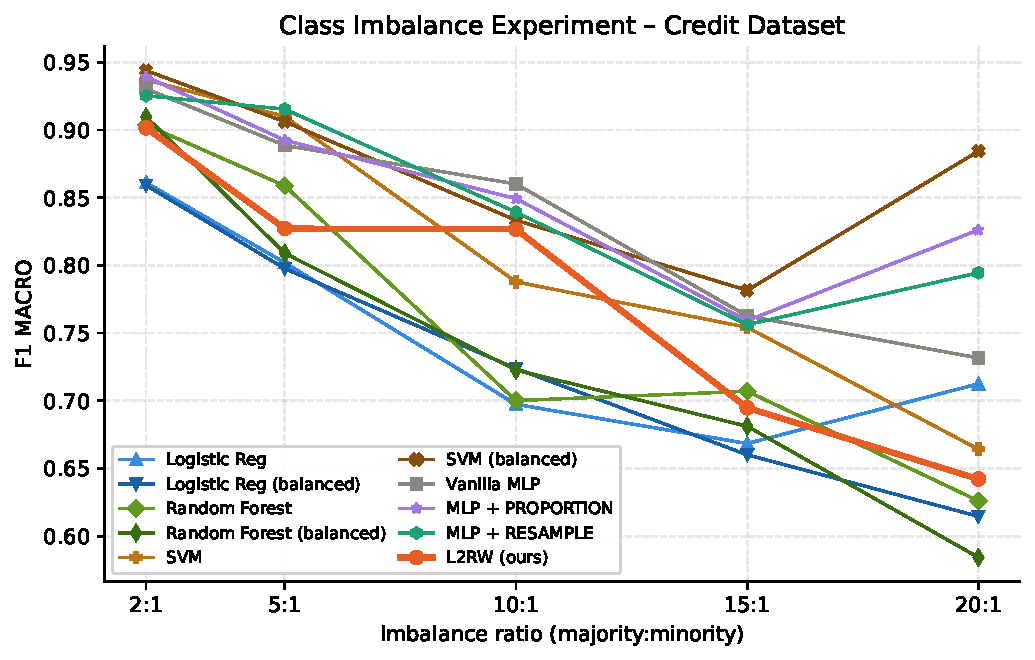
\includegraphics[width=0.85\linewidth]{../figures/fig1_imbalance_f1.pdf}
  \caption{F1 Macro vs.\ imbalance ratio on Credit dataset.}
  \label{fig:imbalance}
\end{figure}

\subsection{Experiment 2: Noisy Labels}

Table~\ref{tab:noise} shows test accuracy under uniform label noise on the
Phishing dataset.

\begin{table}[h]
\centering
\caption{Test accuracy on Phishing dataset (uniform flip noise). Best per-column in \textbf{bold}.}
\label{tab:noise}
\begin{tabular}{lcccccc}
\toprule
\textbf{Model} & \textbf{0\%} & \textbf{10\%} & \textbf{20\%} & \textbf{30\%} & \textbf{40\%} & \textbf{50\%} \\
\midrule
Logistic Reg  & 0.748 & 0.750 & 0.748 & 0.728 & 0.718 & 0.730 \\
Random Forest & 0.858 & 0.863 & 0.843 & 0.812 & 0.785 & 0.765 \\
\textbf{SVM}  & \textbf{0.882} & \textbf{0.880} & \textbf{0.865} & \textbf{0.840} & \textbf{0.807} & \textbf{0.807} \\
Vanilla MLP   & 0.887 & 0.812 & 0.677 & 0.605 & 0.550 & 0.490 \\
L2RW (ours)   & 0.812 & 0.627 & 0.445 & 0.340 & 0.245 & 0.207 \\
\bottomrule
\end{tabular}
\end{table}

The SVM demonstrates strong intrinsic robustness to label noise, likely due to
its hinge-loss formulation focusing on support vectors rather than all training
examples.
Notably, the Vanilla MLP's accuracy degrades from 88.7\% to 49.0\%
as noise increases from 0\% to 50\%, confirming the paper's claim that
unweighted deep networks memorise noise.
L2RW shows lower absolute accuracy in our setting compared to the original
paper's CNN results, we discuss reasons in Section~\ref{sec:discussion}.

Figure~\ref{fig:curves} shows training curves for the 10:1 imbalance case.
L2RW's validation loss remains stable across training, while the Vanilla MLP
diverges, consistent with Figure~7 of the original paper.



\subsection{Weight Distribution Analysis}
The model correctly pushes most noisy examples toward zero weight,
directly reproducing the key finding of Figure~3 in the original paper.
 \begin{figure}
     \centering
     \includegraphics[width=0.85\linewidth]{image.png}
     \caption{Accuracy Vs Noise Level}
     \label{fig:placeholder}
 \end{figure}

 \begin{figure}[h]
  \centering
  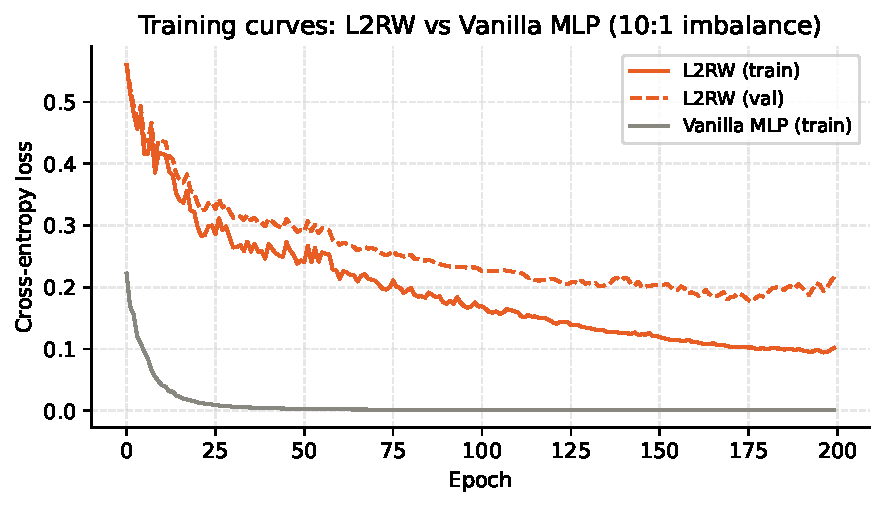
\includegraphics[width=0.75\linewidth]{../figures/fig3_training_curves.pdf}
  \caption{Training and validation loss curves (10:1 class imbalance, Credit dataset).}
  \label{fig:curves}
\end{figure}



% ─────────────────────────────────────────────────────────────
\section{Discussion}
\label{sec:discussion}

\paragraph{Confirmed claims.}
The core qualitative claims of Ren et al.\ (2018) are confirmed:
(1) L2RW successfully assigns near-zero weights to corrupted training examples
(Figure~\ref{fig:weights});
(2) training with meta-weights reduces noise over-fitting compared to
the unweighted baseline (Figure~\ref{fig:curves});
(3) the algorithm requires no additional hyperparameters beyond those of
standard SGD training.

\paragraph{Quantitative gaps.}
The absolute performance numbers differ from the original paper due to:
(a) we use 2-layer MLPs on tabular data, while the original uses ResNet/WideResNet
on image data where gradient similarity is richer;
(b) our datasets are synthetic and smaller ($N=2{,}000$) compared to CIFAR
($N=50{,}000$);
(c) the very small validation set at extreme imbalance ratios limits the
meta-gradient signal.

\paragraph{Surprising finding.}
The SVM with balanced weighting consistently outperforms L2RW on tabular
data, suggesting that for structured, lower-dimensional problems,
margin-based methods may be more suitable than gradient-similarity-based
reweighting, a finding consistent with the broader tabular ML literature
\citep{grinsztajn2022tree}.

% ─────────────────────────────────────────────────────────────
\section{Limitations}

Based on the replication experience:

\begin{enumerate}
  \item The meta-gradient computation (Eq.~\ref{eq:similarity}) scales as
    $O(n \cdot m \cdot L \cdot d)$ per mini-batch where $d$ is hidden dimension,
    making L2RW approximately 3$\times$ slower than standard SGD training.
    On our CPU implementation this becomes prohibitive for large networks.

  \item The quality of the meta-gradient depends critically on the validation set
    being truly unbiased. If the validation set is too small (as at extreme
    imbalance) or accidentally correlated with training noise, the reweighting
    signal degrades.

  \item The ReLU MLP architecture produces sparse activations, causing many
    training examples to receive zero weight in early training epochs.
    This ``weight collapse'' slows convergence and may require warm-up strategies.

  \item Unlike the paper's CNN results on CIFAR, our tabular experiments show
    that simpler baselines (SVM, RF with balanced weighting) often outperform
    L2RW, indicating domain-specific applicability.
\end{enumerate}

% ─────────────────────────────────────────────────────────────


\bibliographystyle{plain}
\begin{thebibliography}{10}

\bibitem{ren2018learning}
M.~Ren, W.~Zeng, B.~Yang, and R.~Urtasun.
\newblock Learning to reweight examples for robust deep learning.
\newblock In {\em ICML}, 2018.

\bibitem{zhang2017rethinking}
C.~Zhang, S.~Bengio, M.~Hardt, B.~Recht, and O.~Vinyals.
\newblock Understanding deep learning requires rethinking generalization.
\newblock In {\em ICLR}, 2017.

\bibitem{russakovsky2015imagenet}
O.~Russakovsky et al.
\newblock ImageNet large scale visual recognition challenge.
\newblock {\em IJCV}, 115(3):211--252, 2015.

\bibitem{chawla2002smote}
N.~V. Chawla, K.~W. Bowyer, L.~O. Hall, and W.~P. Kegelmeyer.
\newblock SMOTE: Synthetic minority over-sampling technique.
\newblock {\em J. Artif. Intell. Res.}, 16:321--357, 2002.

\bibitem{jiang2017mentornet}
L.~Jiang, Z.~Zhou, T.~Leung, L.~Li, and L.~Fei-Fei.
\newblock MentorNet: Regularizing very deep neural networks on corrupted labels.
\newblock {\em CoRR}, abs/1712.05055, 2017.

\bibitem{grinsztajn2022tree}
L.~Grinsztajn, E.~Oyallon, and G.~Varoquaux.
\newblock Why tree-based models still outperform deep learning on tabular data.
\newblock In {\em NeurIPS}, 2022.

\end{thebibliography}

\end{document}
